\subsection{Peripheral Component Interconnect Express (\gls{pcie})}
The \say{Peripheral Component Interconnect (PCI)} architecture has emerged out to be a very thriving beyond even the many more optimistic prospects. Today about every new computer system arrives equipped with at least one PCI slots. Even though there are about to countless PCI slots are shipped globally, there does exists tons of PCI adapter cards which are available to fulfill the all the virtual possible application needs.

This fast growing generation has also raised the demand for many new higher performance interface for input-output communication to support rising technology such as ultra high bandwidth technologies like $ 10-Gb $ Ethernet, $ 10-Gb $ \say{FibreChannel}, $ 12X $ InfiniBand and many more. A regulation which could adapt to carrying out these high performance objectives, while withholding compatibility for previous generation of PCI would beyond any doubt can offer the idealistic solution.

\say{PCI-X 2.0} standard has been developed to meet these objectives. It is capable to serve the uninterrupted performance to feed the nearly all high-bandwidth programs while at the same instance keeping up the full hardware and software backward compatibility for previous \say{PCI} and \say{PCI-X} generations. The PCI-X 2.0 regulation establishes two new grades of speed and performance which are PCI-X 266 and PCI-X 533. These speed grades endeavors bandwidths that are twice and fourfold that of previous generation PCI-X 133 which results to finally supplying bandwidths which are $ 32x $ faster compared to the older version of PCI. It successfully succeeds to bring of additional required performance via time-proven \say{Double Data Rate (DDR)} and \say{Quad Data Rate (QDR)} mechanisms that transmit data at either twice or fourfold the base frequency of clock. As the PCI-X 2.0 conserves too many modules of previous generation PCI it's beneficiary for terrific amount of preceding development job. The OS, device drivers, protocols, connectors, form factor, BIOS, electrical signals, Bus functional modal among many more original PCI modules are all greatly rendered in the new PCI-X 2.0 specification.
Also, many of these modules actually remains untouched in PCI-X 2.0. Due to not having the much of the dissimilarity, it enables development easier because these modules have been already designed and developed with required engineering and familiar to the developers. As a end result, risk is dramatically decreased because the time-to-market became short.

\subsubsection{Functional Description}
The hardware which is used to implement a PCI based system consumes a software interface served by PCI BIOS feature. It has elementary use to generate operations in address spaces specific to PCI (PCI configuration space \cite{pci-config-space}).

The X86 architecture allows following mode to operate as per PCI BIOS features:
\begin{itemize}
  \item Real mode
  \item Protected mode
    \begin{itemize}
      \item $ 286 $ protected mode $ (16:16) $
      \item $ 386 $ protected mode $ (16:32) $
    \end{itemize}
  \item Flat mode (0:32 protected mode)
\end{itemize}
In the Flat mode, all the segments begun at linear address $ 0 $ and span till the end of the whole $ 4-GB $ address space.

\subsubsection{BUS Performances and Number of Slots Compared}
The several architectures characterized by the PCI-SIG\cite{pcisig}. Figure \ref{fig:comparison-of-bus-frequency-bandwidth-slots} portrays the development of PCI bus clock frequencies and bandwidths. Its pretty obvious that the increasing the bus frequency does comprise the load in terms of electrical nodes as also to the maximum permissible connectors on a bus at that clock frequencies.

\begin{figure}[!htbp]
	\centering
	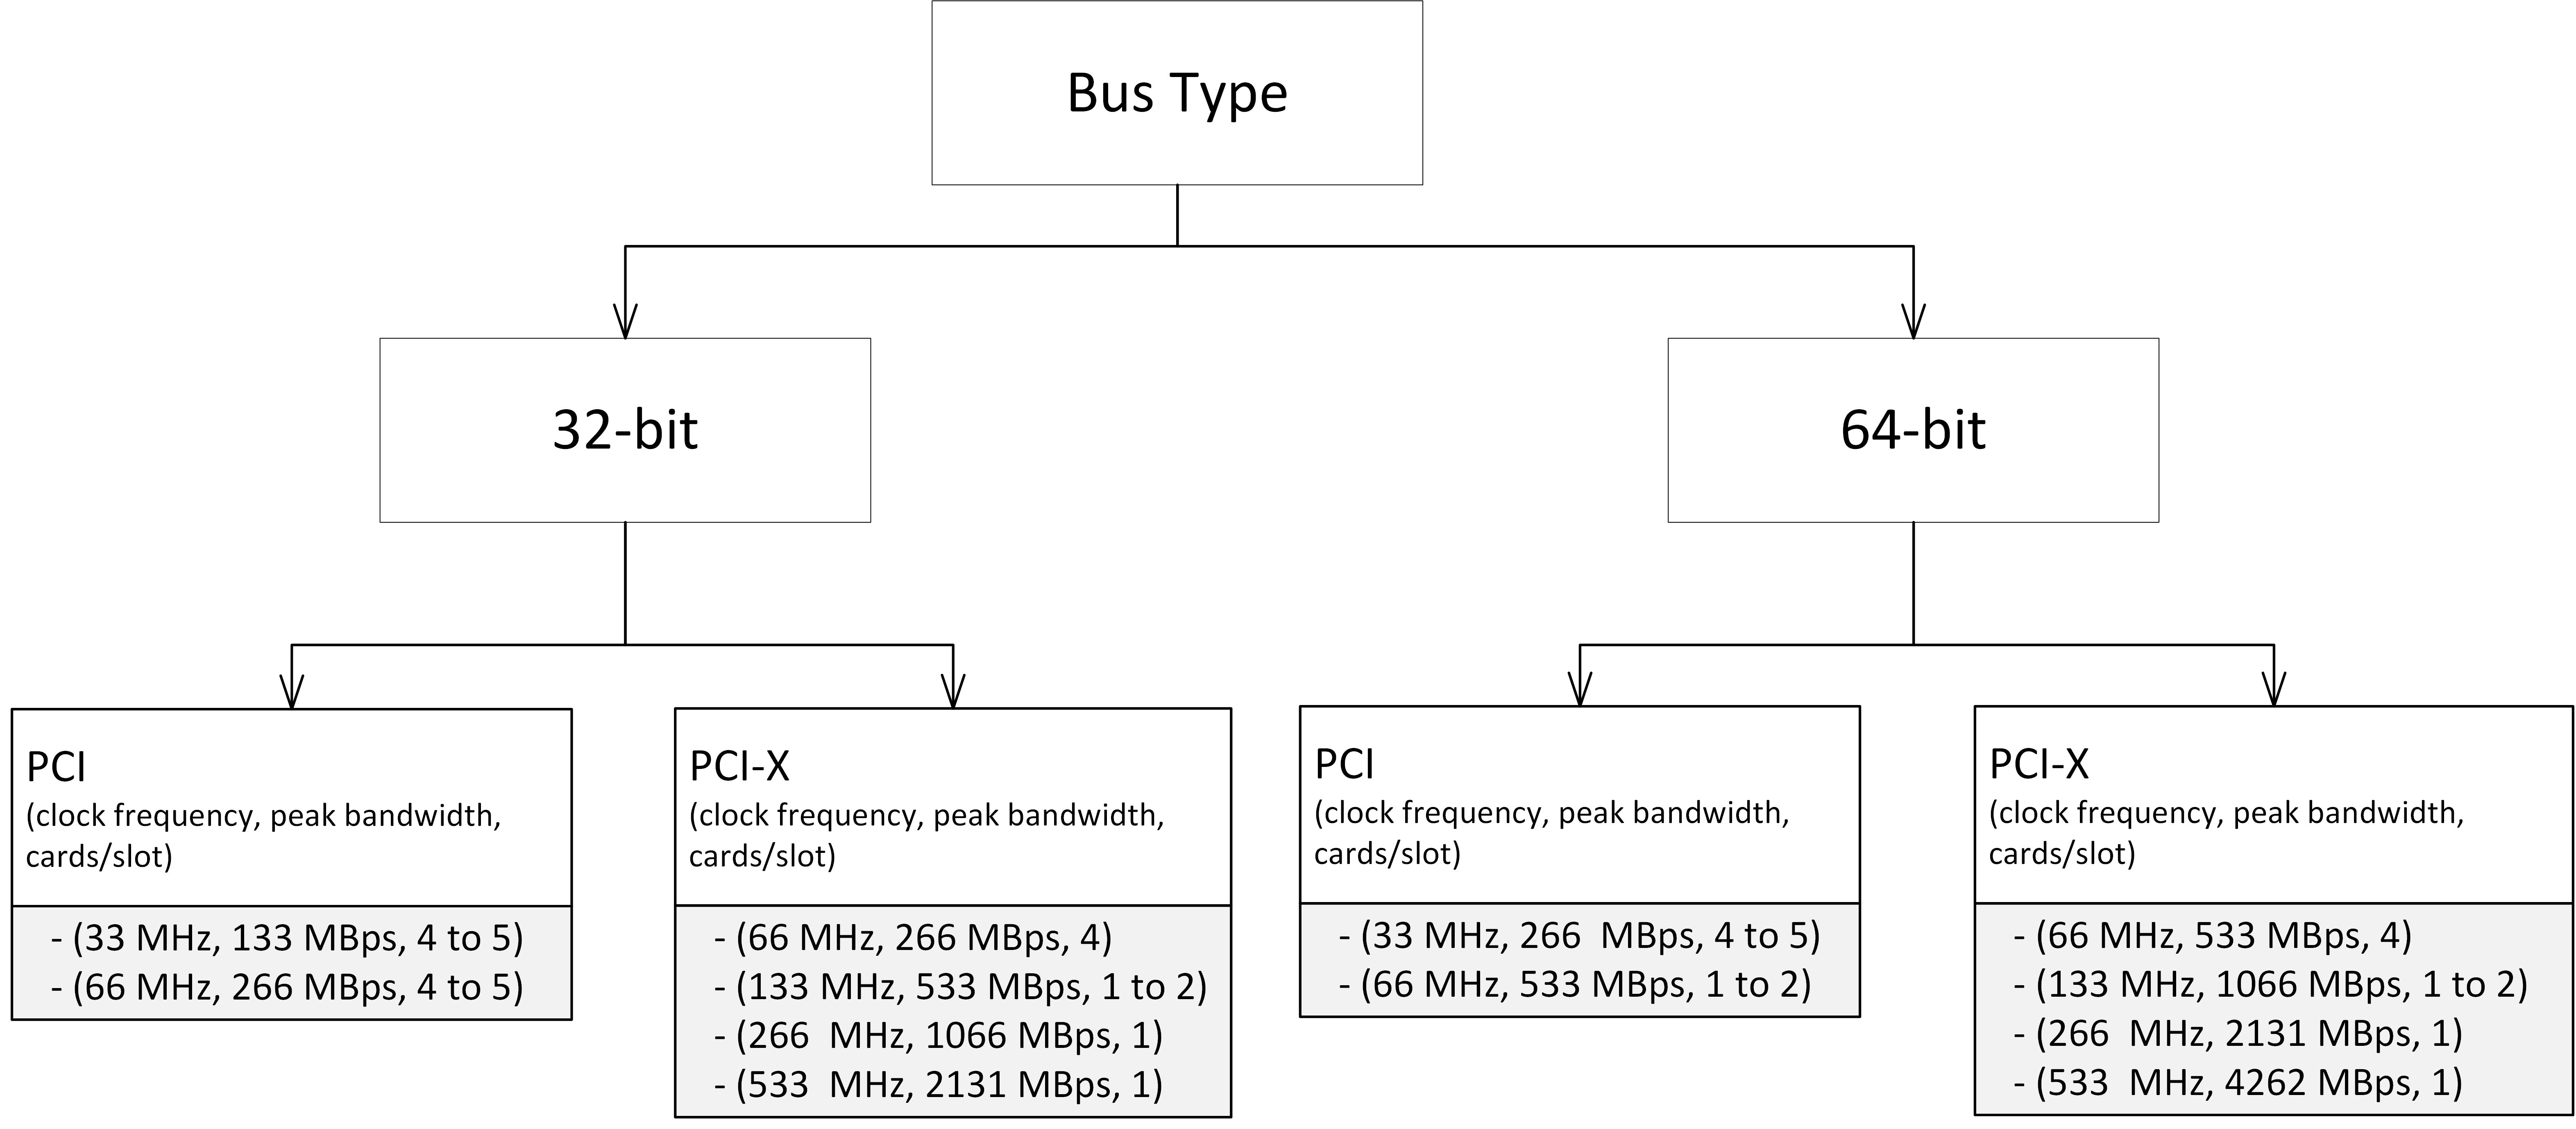
\includegraphics[width=\linewidth]{introduction/comparison-of-bus-frequency-bandwidth-slots}
	\caption{Comparison of Bus Frequency, Bandwidth and Number of Slots}\label{fig:comparison-of-bus-frequency-bandwidth-slots}
\end{figure}

A \say{PCI express (PCIe) Interconnect} is responsible in connecting two PCI devices via PCI link. A PCI link consists if any signal pairs in each direction. These signals ($ x1, x2, x4, x8, x12, x16, x32 $) known as the Lanes. A BIOS designer decides that how many Lanes implementation should be permissible based on the benchmark performance of targeted platform on a given PCI link.
